\chapter{Design} \label{cap:cap3}

\section{Persistance design}
<Identify the product whose software requirements are specified in this document, including the revision or release number. Describe the scope of the product that is covered by this SRS, particularly if this SRS describes only part of the system or a single subsystem.>

\section{MVC modeling}
<Describe any standards or typographical conventions that were followed when writing this SRS, such as fonts or highlighting that have special significance. For example, state whether priorities  for higher-level requirements are assumed to be inherited by detailed requirements, or whether every requirement statement is to have its own priority.>

\subsection{MVC structure}
\subsection{MVC behaviour}

\subsection{BCE Diagrams} \label{sec:BCE}
This paragraph illustrates the BCE pattern representing the architecture that we'll implement in order to develop the WeatherCal system. When identifying the elements for some scenario of system behavior, we can align each participating element with one of three key perspectives : Boundary, Control and Entity. \\This  pattern is a variation of the MVC pattern indeed we can consider mapping the Boundary with the MCV's View, the Control with the MCV's Controller and the Entity with the MVC's Model. Moreover the BCE pattern is not solely appropriate for dealing with user interfaces but it gives also to the controller a slightly different role to play.\\Let's take a deeper look in to the BCE pattern:\begin{itemize}
\item Entity: are objects representing system data and also they perform behavior organized around some cohesive amount of data.
\item Boundaries: are the objects that interface with system actors and most of the times they lay on periphery of a system. Some boundary elements will be "front-end" elements that accept input from outside the area under design and other elements will be "back-end" managing communication to supporting elements outside the system or subsystem.
\item Control: are the elements that mediate between boundaries and entities and control the flow of the interaction of the scenario. They manage the execution of commands coming from the boundary.
\subsubsection{Entity overview}
The diagram in~\ref{fig:entityovervie} illustrates an overview of all entities involved in our system and how they are related with each other.
 \begin{center}
 \begin{figure}[H]
    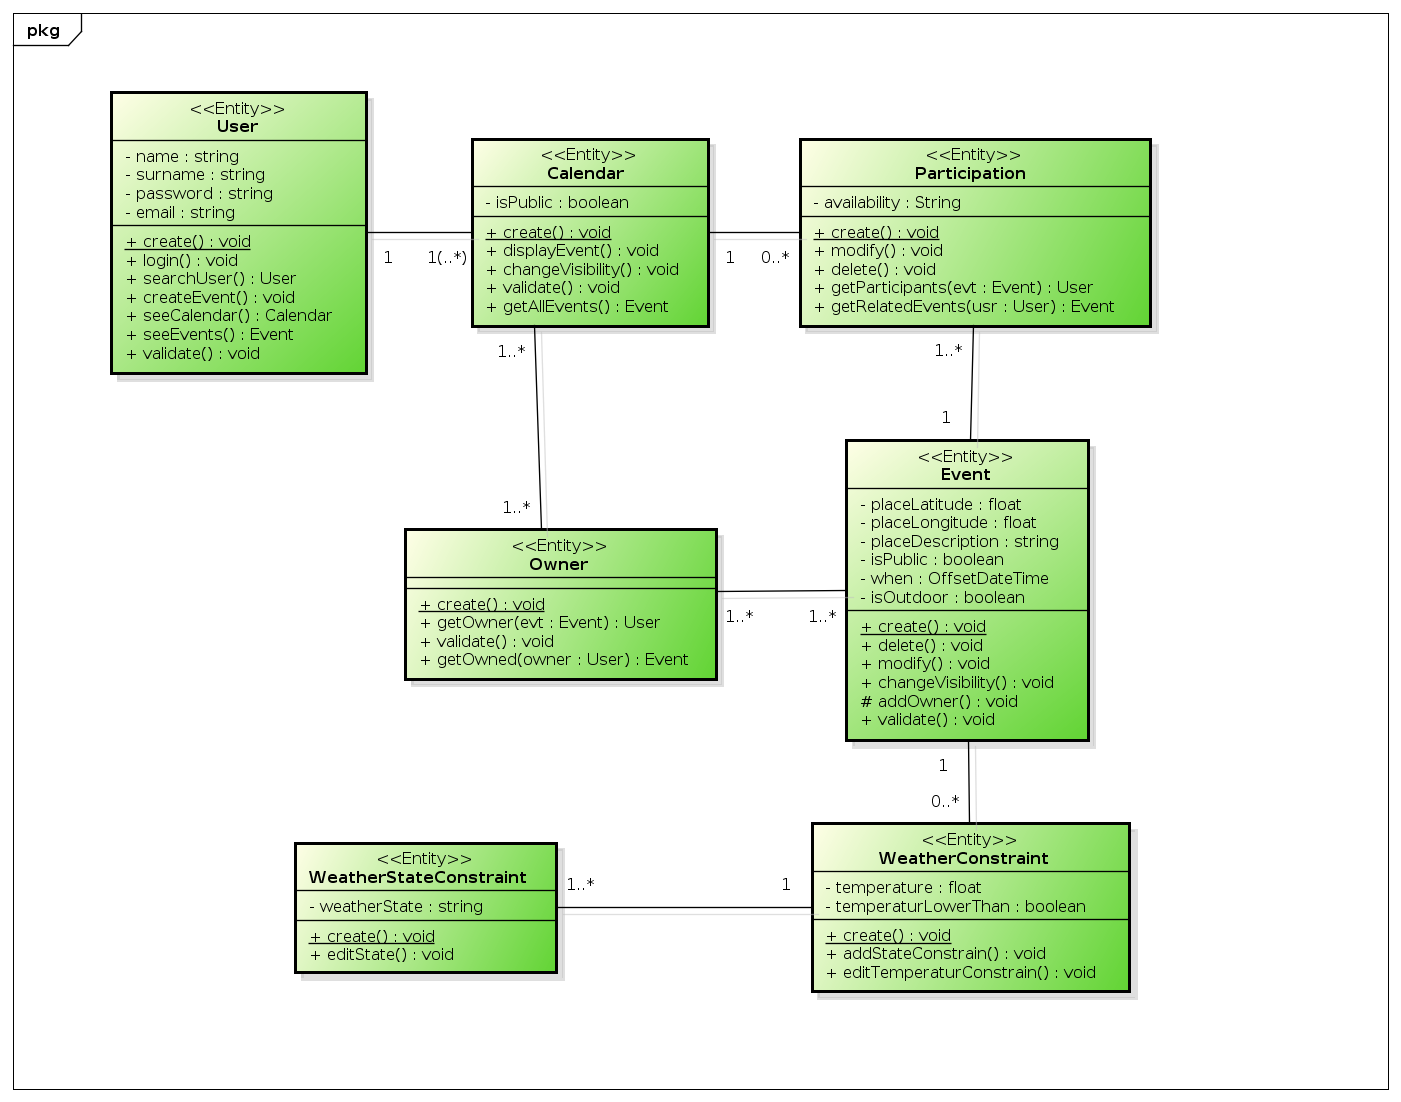
\includegraphics[width=1\textwidth]{../BCEDiagram/BCE/EntityOverview/Entity.png}
    \caption{Entities involved}
     \label{fig:entityovervie}
     \end{figure}
   \end{center}  


\subsubsection{Sign Up and Log In }
The diagram in~\ref{fig:logBCE} shows the flow of the system's behavior related to the registered user's login or to the anonymous user's signup. After the SignUp Controller validates the values submitted by the user, the user reaches his UserPage and then the CalendarController loads its agenda and all associated event. \\In these diagram there are three entities who plays an active role:
\begin{enumerate}
\item  {\bf User}: it's a registered user that can log in to the platform and gets to his UserPage, or he can  represents someone who is not already signed in  to the system and can only reach the main page and register to the platform.
\item  {\bf Event}: represents an event in the calendar. An user can be related to it in two different way, it could be a guest or it could be its owner. Depending on this relation it can perform different action. He can modifies it or creates a new one if he's his owner or change his participation if he's a guest.
\item  {\bf Calendar}: is an element that represents the agenda of an user and contains all his scheduled event. It can be set public or private by its owner.
\end{enumerate}
There are two boundaries involved in this scenario: \begin{enumerate}
\item  {\bf MainPage}: it represents the index page of the system. The one in which a user can either log in or sign up to the platform.
\item  {\bf UserPage}: it stands for the page reached by the user after he logged in. It shows his calendar and all other tasks that the user can performs within it, such as searches for a user, creates or modifies an event or checks for notification.
 \end{enumerate}
The controls who manage the flow of this scenario are two:\begin{enumerate}
\item  {\bf SignUpController}: it's the control whose role is to handle the registration's request of a new user into the system. Whenever a non registered user submits his information the SignUpController verifies the correctness of these information and if they are valid it creates a new User and redirect him to the UserPage.
\item  {\bf LoginController}: his task is to manage the log in of a registered user. It verifies that the credentials submitted by the user are the same provided in the system registration.   
\item  {\bf CalendarController}: It's the responsible for the control of the calendar of an user, it loads it and all its associated events, through it an user can search other users' calendar and view them if they were set as public by their owner.
\end{enumerate}
\begin{center}
 \begin{figure}[H]
    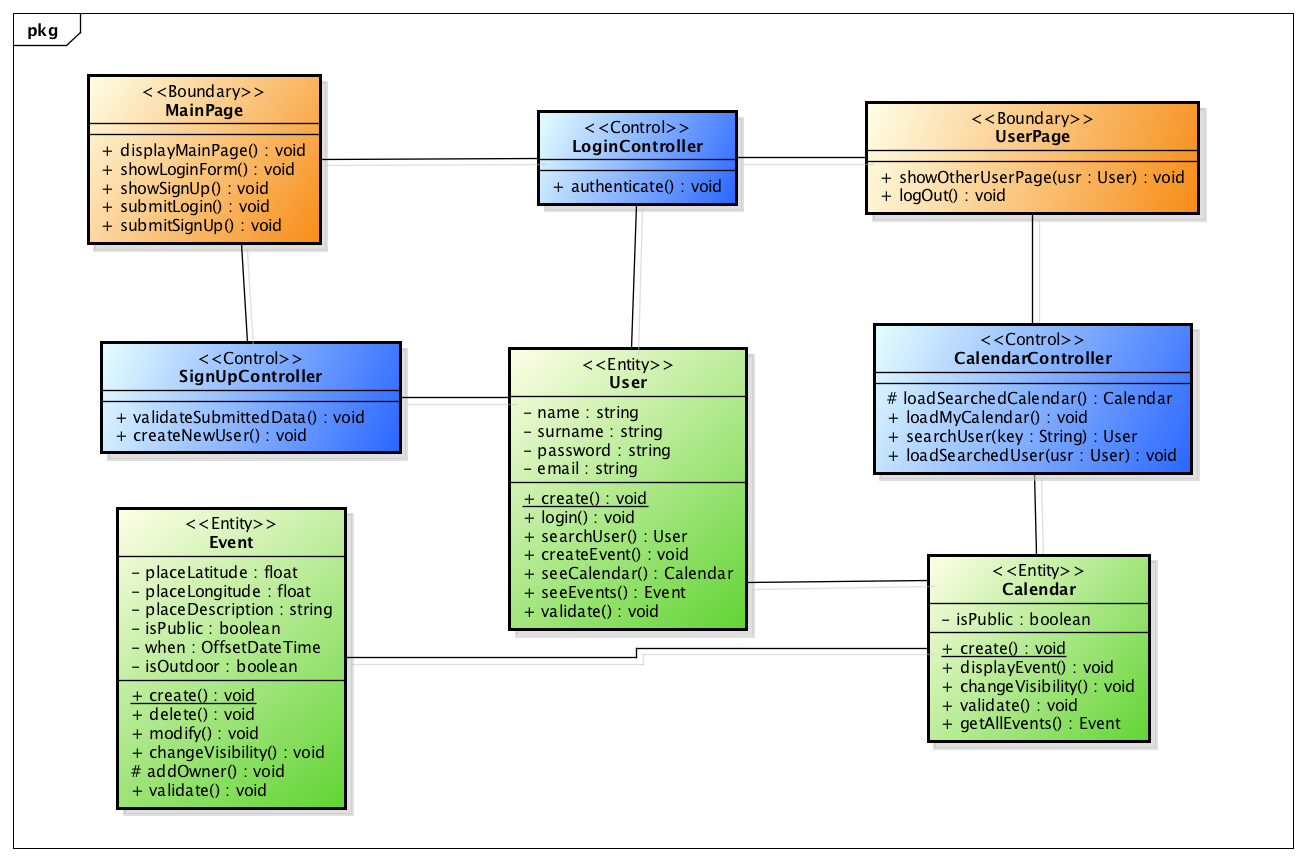
\includegraphics[width=1\textwidth]{../BCEDiagram/BCE/EntityOverview/LoginBCE.png}
    \caption{Sign Up and Log In}
     \label{fig:logBCE}
     \end{figure}
   \end{center}  
\end{itemize}

\subsubsection{Event creation or modification}
The diagram in~\ref{fig:editneweventBCE} illustrates the flow of the creation of the modification of an event. Naturally an user can perform these action only if it's logged in to the system. The top side of the diagram it's related to the log in mechanism already seen in fig~\ref{fig:logBCE} while the bottom side represents the management of an event. From that point on through the EventController a user can either create,delete or modify an event, see the event information or change the participation to it.
\\In these diagram there are only two entities who plays an active role:
\begin{enumerate}
\item  {\bf User}: it's a registered user that can log in to the platform and gets to his UserPage, or he can  represents someone who is not already signed in  to the system and can only reach the main page and register to the platform.
\item  {\bf Event}: represents an event in the calendar. An user can be related to it in two different way, it could be a guest or it could be its owner. Depending on this relation it can perform different action. Modify or create it if it's an owner or change his participation if it's a guest.
\end{enumerate}
There are two boundaries involved in this scenario: \begin{enumerate}
\item  {\bf UserPage}: it stands for the page reach by the user after he logged in. It shows his calendar and all other tasks that the user can performs within it such as searches for a user, creates or modifies an event or checks for notification.
\item {\bf NewModifyEventPage}: is the page that a user uses to create or manipulate an event. It displays all the informations about the selected event such as the place, the date and the desired weather. More over gives to the owner of the event the capability to modify these data or to insert new informations in case that the user is creating a new event.
 \end{enumerate}
The controls who manage the flow of this scenario are two:\begin{enumerate}
\item {\bf LoginController}: his task is to manage the log in of a registered user. It verifies that the credentials submitted by the user are the same provided in the system registration.   
\item {\bf EventController}: this control has several duties many of which concerning the event creation or modification. It's able either to load the information regarding an existing event, to delete an event or to check the correctness of the submitted values for its attributes when the event is created. In addition an invited user to the event can eventually changes the participation to it.
\end{enumerate}
\begin{center}
 \begin{figure}[H]
    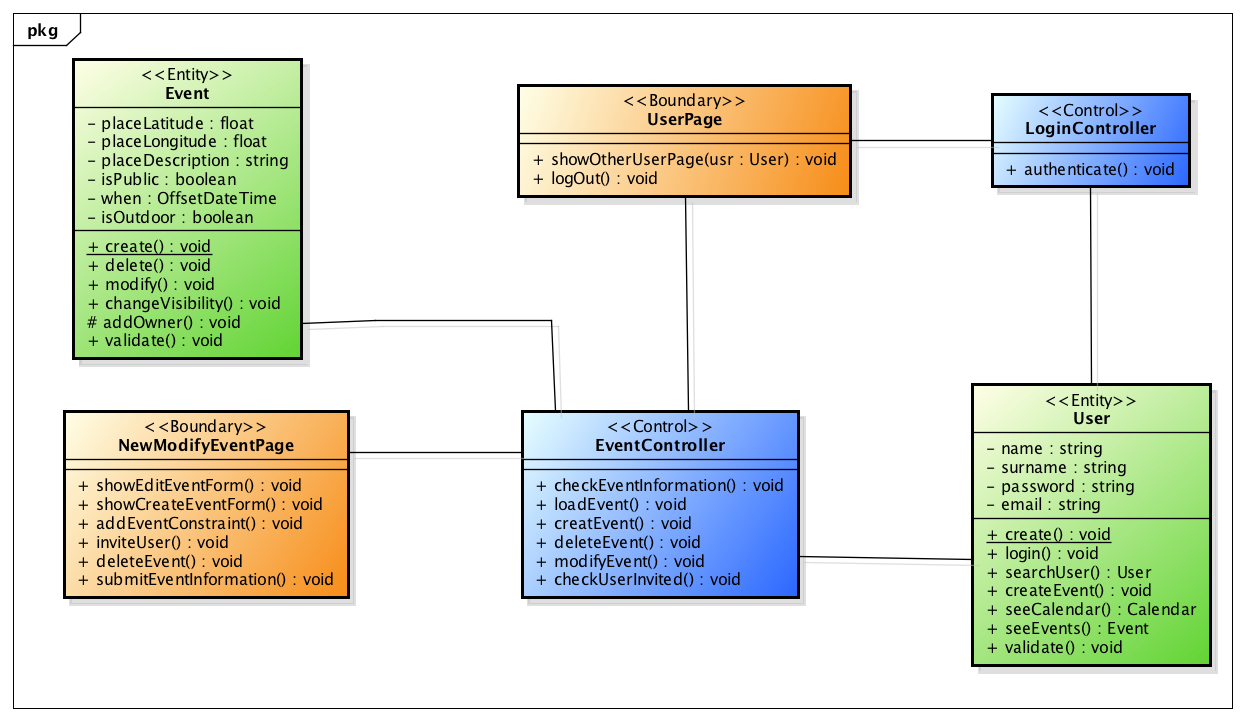
\includegraphics[width=1\textwidth]{../BCEDiagram/BCE/EntityOverview/EventManagementBCE.png}
    \caption{Create or modify an event}
     \label{fig:editneweventBCE}
     \end{figure}
   \end{center}  
\subsubsection{Search Users}
The diagram in fig~\ref{fig:searchBCE} display the scenario involved when a user searches for an other user profile. The flow depends also by the visibility of both the searched calendar and the events within it. This action of course can only be performed by a logged user.\\
In these diagram there are three entities:
\begin{enumerate}
\item  {\bf User}: it's a registered user that can log in to the platform and gets to his UserPage, or he can  represents someone who is not already signed in  to the system and can only reach the main page and register to the platform.
\item  {\bf Event}: represents an event in the calendar. An user can be related to it in two different way, it could be a guest or it could be its owner. Depending on this relation it can perform different action. Modify or create it if it's an owner or change his participation if it's a guest.
\item {\bf Calendar}: is an element that represents the agenda of an user and contains all his scheduled event. It can be set public or private by its owner.
\end{enumerate}
There are two boundaries involved in this scenario: \begin{enumerate}
\item {\bf UserPage}: it stands for the page reach by the user after he logged in. It shows his calendar and all other tasks that the user can performs within it such as searches for a user, creates or modifies an event or checks for notification.
 \item {\bf OtherUserCalendarPage}: is the page that an user can reach after he searched for an other user, depending on the searched user's calendar's visibility it can shows either the calendar itself and its related event or a redirect to the home page
 \end{enumerate}
The controls who manage the flow of this scenario it's unique:\begin{enumerate}
\item  {\bf CalendarController}: It's the responsible for the control of the calendar of an user, it loads it and all its associated events, through it an user can search other users' calendar and view them if they were set as public by their owner.

\end{enumerate}
\begin{center}
 \begin{figure}[H]
    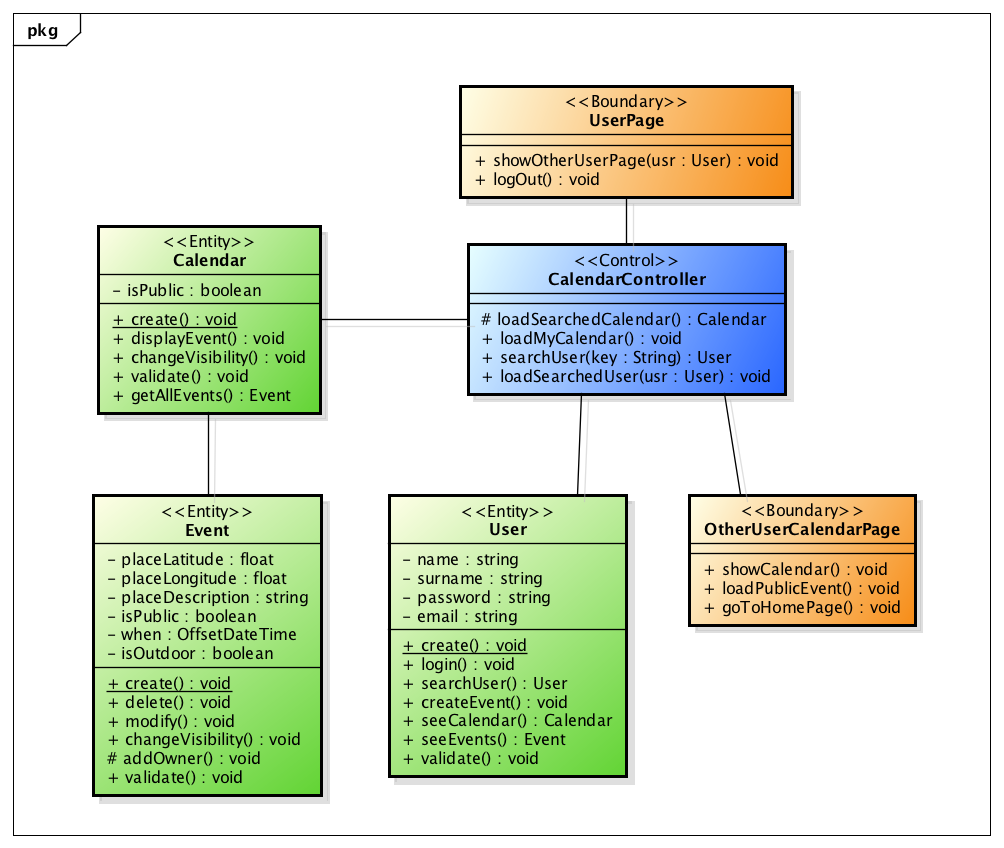
\includegraphics[width=1\textwidth]{../BCEDiagram/BCE/EntityOverview/SearchUserBCE.png}
    \caption{Search users}
     \label{fig:searchBCE}
     \end{figure}
   \end{center}  
\section{Sequence Diagram}
In this section we'll show some sequence diagram associated with the BCE Diagram explained in ~\ref{sec:BCE} section in order to give  a more comprehensive overview either of the BCE patterns and of course of our system behavior.
\subsection{Sign Up}
Figure ~\ref{fig:signupSeq} shows the process for the registration of a new user into the system. As a user accesses the system through the MainPage, he will reach either the login or the register form to the system. If the user wants to register this is what happens.
The user will submit his information through the form and the SignUpController will check that the correctness of the value. If these information are valid then a new user will be created by the SignUpController and inserted in to the system else if the information are not correct a excepetion is thrown and the registration fails. 
\begin{center}
 \begin{figure}[H]
    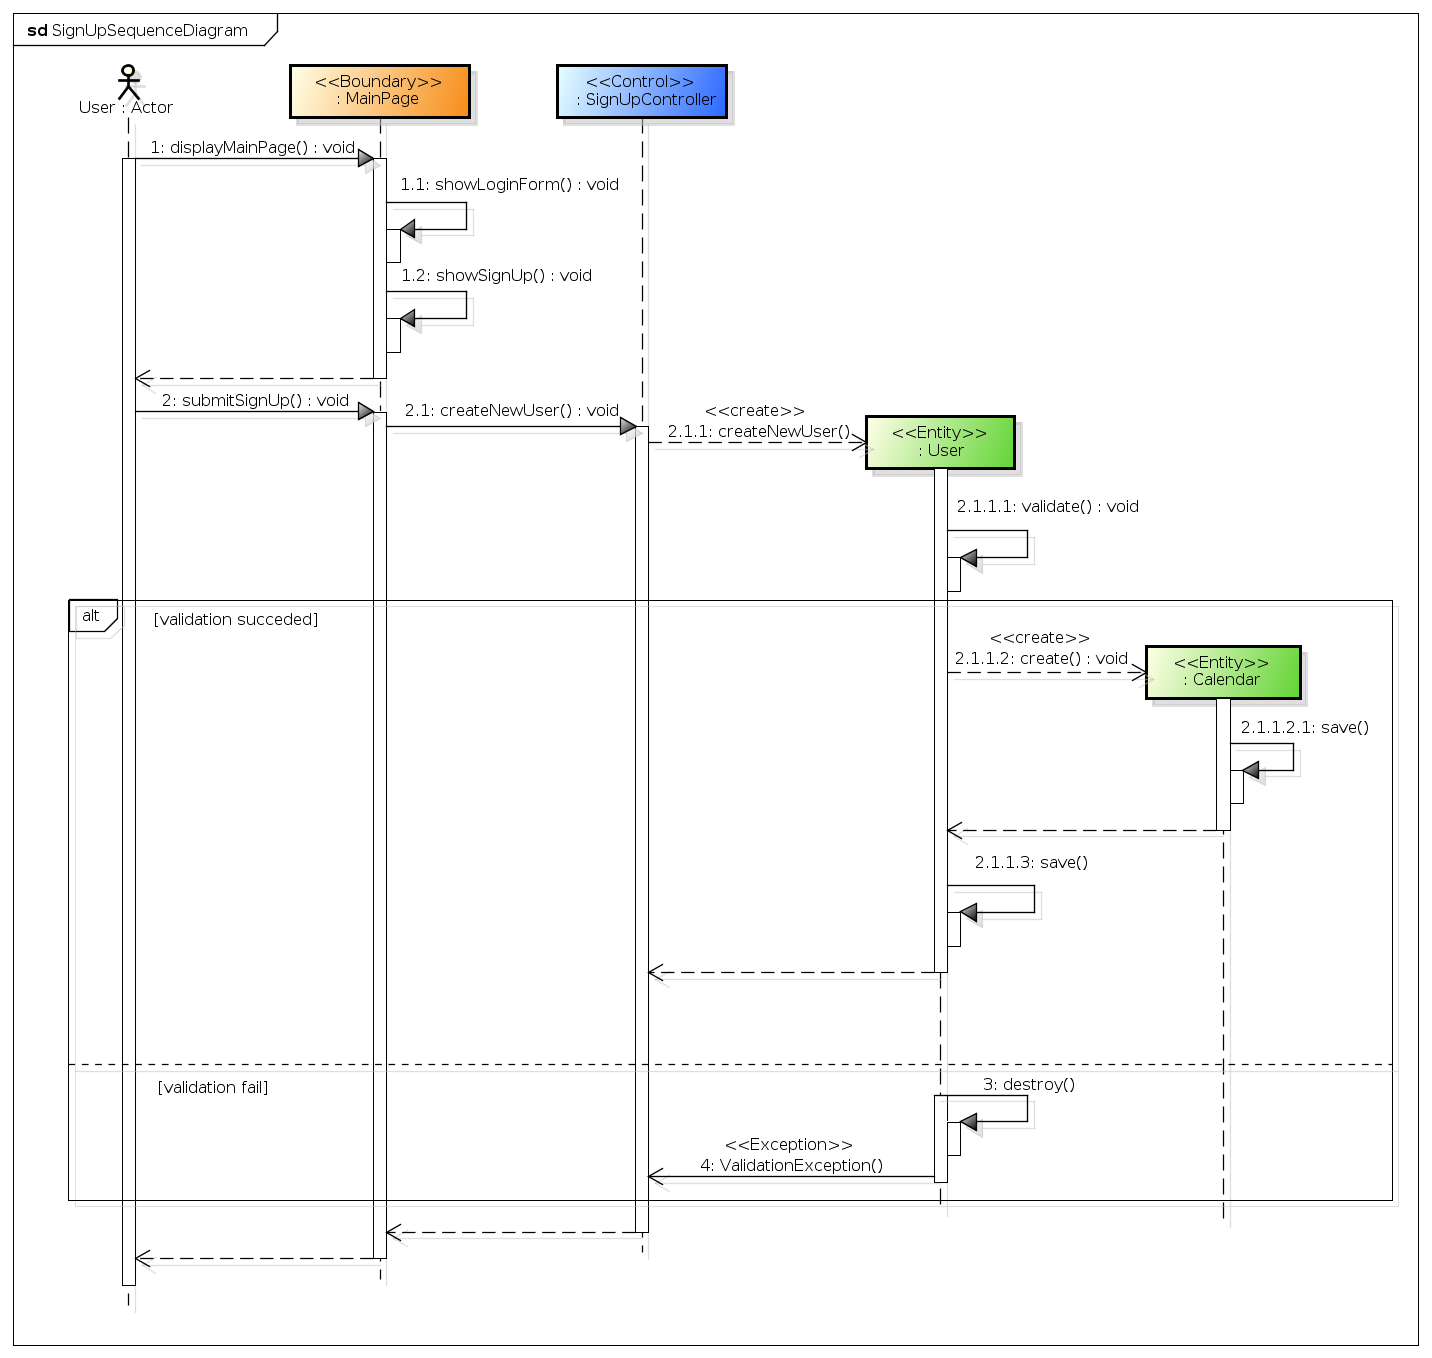
\includegraphics[width=0.9\textwidth]{../BCEDiagram/BCE/EntityOverview/SignUpSequenceDiagram.png}
    \caption{Sign up sequence diagram}
     \label{fig:signupSeq}
     \end{figure}
   \end{center}  
  
  \subsection{Log In}
  The diagrams represented in figure ~\ref{fig:Login1Seq}  and ~\ref{fig:Login2Seq} describe the login phase for a registered user in the system. As the user enters the platform the login form is shown to him and the validation process begins. The whole sequence diagram is divided in two part in order to  give a better understanding of it.\\
  The first diagram fig.~\ref{fig:Login1Seq} refers to the validation of an user. After he submitted his login value, from the log in form in the MainPage, the LoginController verify the validity of these information, in case of an affermative response then the user is authenticated in to the system and he is redirect to the UserPage where thanks to CalendarController his calendar is loaded and shown.
  \begin{center}
 \begin{figure}[H]
    \includegraphics[width=0.9\textwidth]{../BCEDiagram/BCE/EntityOverview/LoginPt1.png}
    \caption{Login part 1}
     \label{fig:Login1Seq}
     \end{figure}
   \end{center}  
     \begin{center}
So if the diagram~\ref{fig:Login1Seq} represents the authentication process of an user then the diagram~\ref{fig:Login2Seq} represents the process used by the system to load the event related to the user's calendar. Once the user is logged in, he can see all the events which owns, all the events in which was invited or all the events that is going to attend. 
 \begin{figure}[H]
    \includegraphics[width=1\textwidth]{../BCEDiagram/BCE/EntityOverview/LoginPt2.png}
    \caption{Login part 2}
     \label{fig:Login2Seq}
     \end{figure}
   \end{center} 
 \subsection{New Event}
 The diagram represented in figure ~\ref{fig:newEveSeq} shows how an user will create a new event and customize it as he wants. The NewModifyEventPage will show to him an empty form to fill with the desired value for the event such as the date, the place, the invited user or the weather constraint. The same form is shown to an user that wants to see the event's details and eventually ,if he's also its owner, to modify the current value.
Therefore after an user creates or modifies an event, the EventController check that all the values are correct and then either creates a new event or modify an existing one or, if the submitted preferences are not valid, it throws an exception and the creation process fails.  
  \begin{center}
 \begin{figure}[H]
    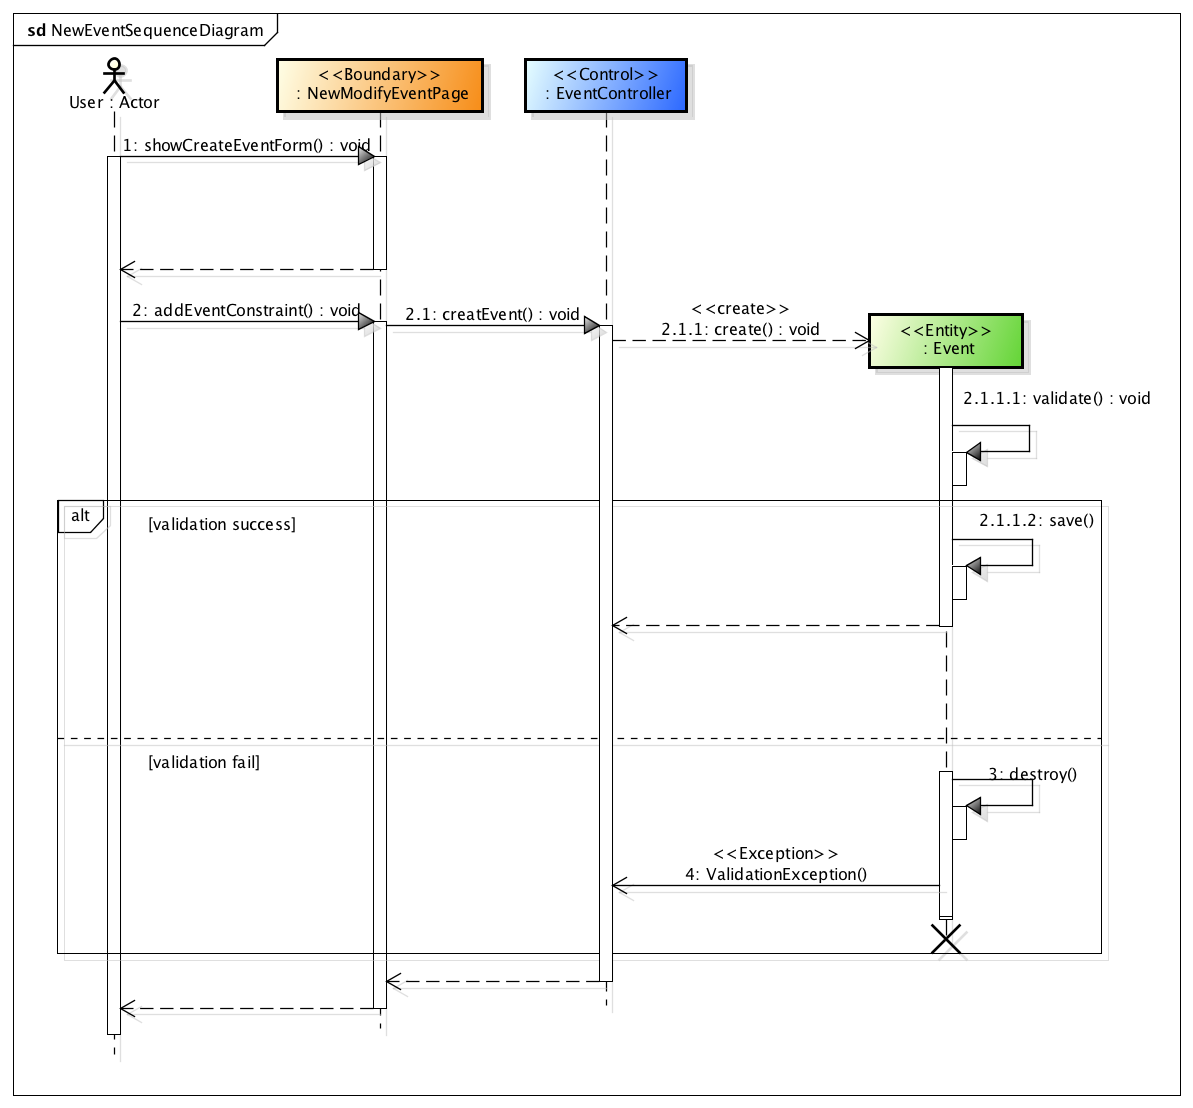
\includegraphics[width=1\textwidth]{../BCEDiagram/BCE/EntityOverview/NewEventSequenceDiagram.png}
    \caption{New event sequence Diagram}
     \label{fig:newEveSeq}
     \end{figure}
   \end{center} 
\subsection{Search Users}
The diagram in figure ~\ref{fig:searchusSeq} shows the behavior of the system when an user searches for an other user's agenda. The searching and the loading process of the target calendar is accomplished by the CalendarController which once it finds the calendar and makes sure that it was marked visible to everyone by its owner, it fetches all the event related to it, taking care to filter the public event and the private one and finally shows to the user only the public event of the desired user.
 \begin{center}
 \begin{figure}[H]
    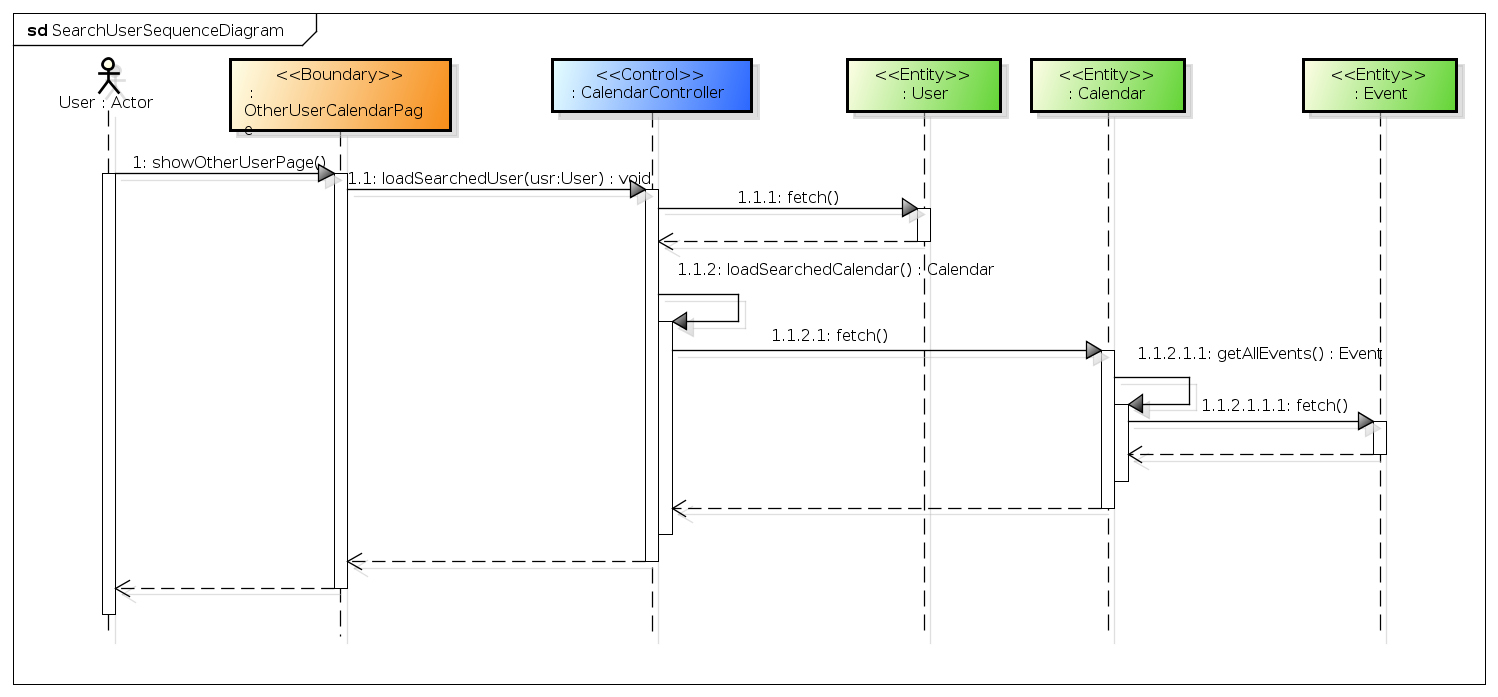
\includegraphics[width=1\textwidth]{../BCEDiagram/BCE/EntityOverview/SearchUserSequenceDiagram.png}
    \caption{Search users sequence diagram}
     \label{fig:searchusSeq}
     \end{figure}
   \end{center} 

